\documentclass{standalone}
\usepackage{ tikz }

\usetikzlibrary{calc}

\begin{document}
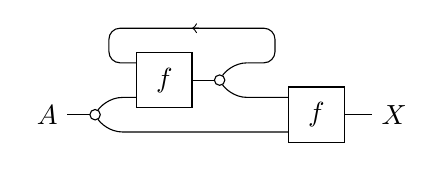
\begin{tikzpicture}[yscale=-1,x=1em,y=1.25em]
        
    \coordinate (O) at (0,0);

    \node [anchor=east] at ($(O)$) {$A$};

    \node (C1) [draw, circle, fill=white, scale=0.4] at ($(O) +(1,0)$) {};

    \node (F1) [draw, minimum height = 2em, minimum width = 2em, fill=white] at ($(C1) +(2.5,-1)$){$f$};
    \coordinate (F1I1) at ($(F1) +(-1,-0.5)$);
    \coordinate (F1I2) at ($(F1) +(-1,0.5)$);
    \coordinate (F1O1) at ($(F1) +(1,0)$);

    \coordinate (MP) at ($(F1) + (1,-1.5)$);

    \node (C2) [draw, circle, fill=white, scale=0.4] at ($(F1) +(2,0)$) {};
    \coordinate (T1) at ($(C2) +(1,-0.5)$);

    \node (F2) [draw, minimum height = 2em, minimum width = 2em, fill=white] at ($(C2) +(3.5,1)$){$f$};
    \coordinate (F2I1) at ($(F2) +(-1,-0.5)$);
    \coordinate (F2I2) at ($(F2) +(-1,0.5)$);
    \coordinate (F2O1) at ($(F2) +(1,0)$);

    \node (X1) [anchor=west] at ($(F2O1) +(1,0)$) {$X$};

    \draw (O) -- (C1);
    \draw (C1) to[out=285, in=180] ($(C1) +(1,-0.5)$) to (F1I2);
    \draw (F1O1) -- (C2);
    \draw (C2) to[out=285, in=180] (T1);
    \draw [->, rounded corners] (T1) -- ($(T1) +(1,0)$) -- ($(T1) +(1,-1)$) -- (MP);
    \draw [rounded corners] ($(MP) + (0.25,0)$) -- ($(F1) +(-2,-1.5)$) -- ($(F1) +(-2,-0.5)$) -- (F1I1);
    \draw (C1) to[out=75, in=180] ($(C1) + (1,0.5)$) to (F2I2);
    \draw (C2) to[out=75, in=180] ($(C2) + (1,0.5)$) to (F2I1);
    \draw (F2O1) to (X1);



\end{tikzpicture}
\end{document}